\chapter{小缓冲区组技术}
\label{chap:sba}

存储介质性能的发展要求比传统系统更轻薄的存储软件栈,以更好地发挥硬件提供的更高的吞吐能力和更低的访问延迟。我们提出将一个可扩展的事务性内存系统直接架构在大容量非易失性存储设备上以达到上述要求。我们的解决方案绕开了复杂的代价高昂的数据库系统,应用程序可直接使用事务;并且解决了传统持久性事务性内存系统在可扩展性和容量方面的局限。系统假设市面上现成的存储设备,并基于我们对最新的接口和存储设备的特性的观察。我们通过两项技术改进了持久性事务性内存系统一致性机制的可扩展性和效率:
(1)采用我们事务性内存系统的\emph{快照隔离}机制使得持久化的开销对只读负载隐藏;
(2)设计了共享的\emph{小缓冲区组技术}供预写式日志使用。该缓冲区设计在满足一致性要求的同时,面向事务性内存系统设计,可以同时实现高吞吐率和低延迟的特性。

\section{可扩展的持久性事务性内存系统}

\subsection{现有系统问题}

存储系统对应用的性能有显著影响。两个硬件发展的新趋势增强了这方面影响。首先,非易失性存储(例如闪存\cite{Chen:2009:UIC:1555349.1555371, 4804997}、ReRAM\cite{6327378, 7168603}、PCM\cite{Loke22062012,6176872,Raoux:2008:PRA,10.1109/MM.2010.24}、STT-RAM\cite{4443191,6557176}等)极大扩展了传统存储系统的带宽,降低了其访问延迟,相应地也要求高效的系统软件来充分利用这些优势。其次,多核和多处理器架构需要存储软件层的可扩展性来匹配上层应用的可扩展性\cite{Zheng:2014:FDF:2685048.2685085,Kimura:2015:FOE:2723372.2746480}。

最初事务性内存系统的提出是用于并发控制,为了简化基于锁的程序的设计和编码。由于持久化的开销较高,传统事务性内存中的事务并不提供持久性的保证,而仅仅保证ACID中的另外三项:原子性、一致性和隔离性。而应用程序需要使用其他事务性系统,例如数据库,来完成数据持久化的需求。这种使用模式和厚重的数据库系统带来可观的系统开销,而且随着高速存储硬件的发展日益成为系统性能的瓶颈。相较于轻量级的事务性内存系统,数据库系统可能带来几十倍的性能降低\cite{Volos:2011:MLP:1950365.1950379,
Coburn:2011:NMP:1950365.1950380}。

因此,完整支持ACID的事务性内存系统,作为应用程序访问持久性数据的新接口,得到广泛的关注和研究\cite{Volos:2011:MLP:1950365.1950379,
Coburn:2011:NMP:1950365.1950380, Zhao:2013:KCP:2540708.2540744, 6828760}。然而,现有的此类系统多依赖于新型的可字节访问的非易失性内存(例如ReRAM、PCM、STT-RAM等)。新型非易失性内存尚未普遍商业应用,在价格、容量等方面有诸多限制(例如Intel-Micro最新推出的3D XPoint非易失性内存单片容量128GB)。而闪存、固态硬盘等按块访问的非易失性存储设备已经非常成熟,价格低廉,在基于PCIe的NVMHCI 或NVMe~\cite{nvme}的最新接口技术下容量和扩展性都更加理想。

\subsection{挑战和应对}

本章提出一种基于当前商业应用的非易失性存储的持久性事务性内存,具备并发能力、吞吐能力和容量的高可扩展性。我们采用预写式日志的方式来实现数据的持久性以及保证持久性数据的一致性,重点改进了缓冲区的设计,解决了持久化及其故障时数据一致性机制的性能瓶颈。

我们面临两方面的挑战。第一,商业可用的非易失性存储,如基于闪存的固态硬盘,虽然容量可扩展性高,但其写入延迟仍然是不可忽略的问题。该延迟比新型的可字节访问的非易失性内存介质要高两个以上的数量级。在一个事务性内存系统中直接应用当前商业可用的非易失性存储并不可行,需要我们将持久化的开销尽量隐藏起来。系统吞吐性能之所以对持久化开销很敏感,原因是写事务需要锁住所有相关的写锁直到其预写式日志项完成持久化。这很容易成为系统性能瓶颈\cite{Chen:2009:FEF:1559845.1559855,
Johnson:2010:ASA:1920841.1920928, Johnson:2012:SWL:2205457.2205463,
Zheng:2014:FDF:2685048.2685085},并且这种由于日志导致的锁行为\cite{Johnson:2010:ASA:1920841.1920928}被广泛定位为线程竞争等待的一个主要原因。第二,传统集中式大体积的日志缓冲区在高并发的使用环境下会导致低效的缓冲区竞争\cite{Johnson:2010:ASA:1920841.1920928,
Huang:2014:NLT:2735496.2735502}。该设计思想主要来自于机械硬盘顺序写性能的突出优势,并不与非易失性存储的特性相符合。采用线程局部的缓冲区\cite{Johnson:2012:SWL:2205457.2205463,
Zheng:2014:FDF:2685048.2685085, Wang:2014:SLT:2732951.2732960}需要单个线程执行多个事务来填充其独占的缓冲区以进行组提交,与事务性内存简单的线程模型相违背。而且,它依然需要不同线程间进行事务级的协调\cite{Johnson:2012:SWL:2205457.2205463,Wang:2014:SLT:2732951.2732960}。

为了应对第一个挑战,我们在事务性内存系统中采用快照隔离技术。特别地,我们维护一致的数据历史版本,只读的事务在一个历史快照上执行,不会与其他事务冲突,可以直接提交。相对于传统将动态写入数据定期归档进数据仓库再进行分析的模式,当前实时性分析与动态写入数据混合的模式\cite{ren2011querying,
Cheng:2012:KTP:2168836.2168846,4302625,Corbett:2012:SGG:2387880.2387905}更能体现出我们系统避免持久化写事务拖累读事务的优势。我们的系统可以显著提高此类负载下的综合吞吐率。

为了应对第二个挑战,我们提出了一种共享的小缓冲区组的设计。这样,多个CPU核并发产生的日志项可以很快地填充满小缓冲区,从而显著减少组提交策略下由于等待缓冲区填充造成的延迟。我们通过将线程顺序循环分布于不同的缓冲区来减少线程间的竞争,避免采用基于阶段或者事件的复杂设计。更重要地,我们只需要粗粒度地维护缓冲区组之间的顺序,而不需要传统上的事务级的协调。

\section{小缓冲区组技术}

\begin{figure}[t]
\centering
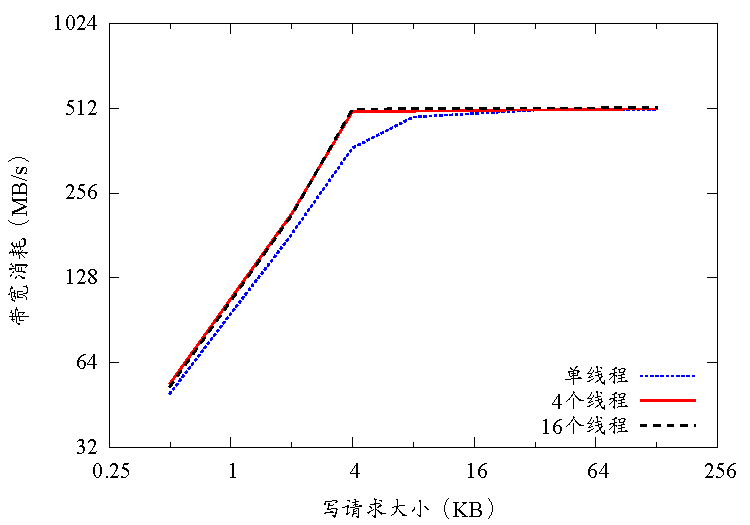
\includegraphics[width=0.9\columnwidth]{figures/nvme-bandwidth}
\caption{基于NVMe接口的Intel固态硬盘在不同写请求大小下的带宽消耗。}
\label{fig-nvme-bandwidth}
\end{figure}

图\ref{fig-nvme-bandwidth}绘制了一台PCIe NVMe接口的英特尔固态硬盘Intel SSD DC P3600在不同写请求大小下的带宽消耗。实验使用一台24核服务器,开启一定数量的线程直接向NVMe块设备连续发送固定大小的写请求。我们可以从曲线中得出两点观察结论。第一,峰值带宽可达到500~MB/s,如果假设512~B的写入请求大小,那么单台设备可支持每秒百万级的事务吞吐率。数据库在相同硬件配置下很难达到相同的吞吐率。第二,使用多个线程时,峰值带宽在写大小超过4~KB后即可达到,表明KB级别的缓冲区大小已经能够饱和利用存储设备性能,而该范围比为传统机械磁盘设计的缓冲区小两个数量级。小缓冲区可以在确认写完成时获得更小的延迟。

\section{系统实现}

\subsection{快照隔离}
\label{subsec:sba-si}

快照隔离在传统数据库和内存系统中即有应用\cite{Daudjee:2006:LDR:1182635.1164189, Fekete:2005:MSI:1071610.1071615, Ports:2012:SSI:2367502.2367523, Litz:2014:SRT:2541940.2541952},其基本过程为:事务执行时首先获得目标数据的一个快照,然后在该快照上执行事务。由于事务所见的数据是一致的和隔离的,其执行结果亦满足一致性和隔离性。而后,系统尝试将事务所做的更改原子地提交到主数据集中。提交过程首先要经历一个\emph{验证}过程,确保该事务的更改与其他事务的更改不冲突。如果冲突则需要选择冲突的一方中止,重新按上述过程再执行。

我们将快照隔离的技术实现在虚拟内存中。这部分工作,基于斯坦福大学计算机系H. Litz和D. Cherition等人开发的ExciteVM系统。由于该系统尚未公开发表,此处仅做基本的背景介绍。该系统的基本实现方式是利用页表和写时拷贝实现获取目标数据的快照。正常情况下,修改页表需要操作系统内核的参与,不仅开销大,而且给系统部署带来麻烦(因为需要重新编译内核)。所幸的是,斯坦福大学的A. Belay等提出的Dune系统\cite{Belay:2012:DSU:2387880.2387913}借助虚拟化技术使得用户态程序可以在不侵害其他程序安全性的情况下自己修改页表。ExciteVM的实现采用了Dune的技术。

\subsection{小缓冲区组}

小缓冲区组的基本数据结构即若干个KB级大小的数组,分别作为各个小缓冲区。所有小缓冲区构成一个循环数组。我们需要维护一个全局的日志序列(LSN)变量,为每个事务分配唯一的ID。我们令该ID等于事务在NVM上的地址,因为NVM的数据组织成日志结构,其末尾地址是单增的。这种ID分配方式的好处在于,我们仅依据ID即可将事务循环顺次分配到各个小缓冲区。这样,事务ID和小缓冲区编号之间建立起静态的映射关系,所以确定事务使用的小缓冲区仅需要获取LSN时的一次原子增操作,而不再需要其他的协调机制。

一个小缓冲区可能被多个线程使用,因为各个事务不同的写大小和小缓冲区固定的大小之间显然是无法对准的。于是,我们需要为每个小缓冲区协调使用它的各个事务线程。具体地,该协调机制需要完成的目标和主要手段如下。
\begin{enumerate}
\item \label{item:dirty-counter} 相关的事务线程需要知道一个小缓冲区何时填满,并在不满时进行等待。为此,我们给每个小缓冲区设置一个局部的原子计数器,来记录缓冲区的使用状况。与此同时,我们采用轻量级的线程库实现线程的等待与唤醒,而非复杂的事件系统。
\item 在一个小缓冲区填满后,需要一个线程负责刷出该缓冲区数据到NVM。为此,我们直接在事务线程被唤醒时任选出其中一个进行最终的数据刷出操作。与第\ref{item:dirty-counter}点设计思想类似,我们不再引入其他事件或着线程来完成刷出任务。在事务性内存系统中,这些事务线程即为应用程序的线程,而不像数据库中工作线程与客户请求的线程相互独立。所以,我们的实现方式与事务性内存的特点相一致。
\item 一个事务线程的写可能跨域两个或多个小缓冲区,需要避免小缓冲区之间相互等待造成的死锁。为此,我们按这样的方式定序:如果一个事务的写跨越两个缓冲区,那么它只负责低地址的小缓冲区刷出,而对于高地址的小缓冲区,它仅将数据填入其中而不负责刷出,也不进行等待;其余情况下,不论小缓冲区被事务独占(即事务写范围完全涵盖一个小缓冲区)还是事务被小缓冲区独占(即小缓冲区接收的范围完全涵盖一个事务的写),该事务均允许负责刷出相应的小缓冲区。
%我们将事务线程对其有权刷出的小缓冲区填充数据的行为称作“填写”,而对其无权刷出的小缓冲区填充数据的行为称作“填补”。
\item 由于各个事务写往小缓冲区组的数据量可能很大,超过小缓冲区组整体刷出数据的速度,所以需要处理小缓冲区构成的循环数组越界的问题。我们没有采用通过全局变量维护循环数组首尾指针的传统方式,因为该方式可能导致多线程对全局变量竞争的瓶颈。相反,我们继续将新来的事务分配到对应的小缓冲区上,从而将并发控制的压力分布到各个小缓冲区。为了保证一个小缓冲区每次刷出的数据属于同一个地址范围,我们为小缓冲区设置了一个标记域。如果一个事务发现其对应的小缓冲区的标记与自身要写的地址不符,则继续等待。
\item 我们需要确定哪些事务的结果可以对读操作可见。我们维护一个全局的地址变量,记录已经刷出的最大的事务ID,即事务ID小于该值的事务已经完成持久化。在ExciteVM中,事务对应着数据的版本。任意时刻,新的事务请求获得快照时,即取该最大事务ID的版本。值得注意的是,我们并不需要在每个事务提交时更改该最大事务ID,而仅需要在每个小缓冲区完成数据刷出时更新该ID。所以,我们只需要做小缓冲区级别而非事务级别的协调。
\item 当一组负载的运行接近结束时,会出现少数剩余线程无法填满小缓冲区的情况。所以我们仍然需要像传统大缓冲区一样设置超时监控。如果一个小缓冲区在一定时间内不再收到新的写,那么该缓冲区会自动选取正在等待的一个事务线程执行数据刷出操作。
\end{enumerate}

\section{性能评测}

\subsection{基准测试集}

我们选用了YCSB(Yahoo! Cloud Serving Benchmark)\cite{Cooper:2010:BCS:1807128.1807152}作为我们的基准测试集。然而原版测试集基于Java实现,与我们的静态库冲突。为此,我们将YCSB整体移植到C++语言。我们C++版的YCSB基准测试集在\url{https://github.com/basicthinker/YCSB-C}开放源代码。

具体地,YCSB包含如下六个测试负载类型,后文的实验结果分析需要对此有所了解。
\begin{itemize}
\item 负载A:更新操作密集型。包含比例为50:50的读和写请求。典型应用场景:记录用户最近活动的会话存储(session store)。
\item 负载B:读操作密集型。包含比例为95:5的读和写请求。典型应用场景:图片的标记。
\item 负载C:只读类型。典型应用场景:用户信息缓存。
\item 负载D:读最近数据的类型。新的记录被插入,而最新的记录被读得最多。读和写请求的比例是95:5。典型应用场景:用户状态更新。
\item 负载E:范围查询型。不同于如上只做个体记录操作的类型。扫描和插入请求的比例是95:5。典型应用场景:处理用户对话记录。
\item 负载F:读改写类型。记录首先被读出,作出修改后再插入回去。典型应用场景:用户数据库。
\end{itemize}

\subsection{实验环境}

承载本章实验的服务器使用Intel Xeon CPU E5-2670(16个物理核)以及64 GB内存。在YCSB的每组测试前,数据集中预置10万条记录。每个记录由若干100字节的域构成。

\subsection{对照系统}

对照系统主要基于英特尔线程库Intel Threading Building Blocks(简称为TBB)和C++标准库STL实现,共包含如下几种组合。

\begin{itemize}
\item Lock-STL:基于STL的unordered\_map实现的内存中键值存储,使用全局互斥锁做并发控制。
\item TBB-unordered:基于TBB的concurrent\_unordered\_map\cite{TBB:concurrent-unordered-map}实现的内存中键值存储,使用读写锁保护删除操作。
\item TBB-hash:基于TBB的concurrent\_hash\_map\cite{TBB:concurrent-hash-map}实现的内存中键值存储,使用读写锁保护扫描查询操作。
\item Excite:基于ExciteVM和小缓冲区组实现的内存中键值存储。

\end{itemize}

\begin{table}[!ht]
\caption{在本系统实现上运行YCSB负载A的事务延迟分析。}
\label{tab:sba-micro}
\centering
\begin{tabular}{|c|c|c|c|c|}
\hline
线程数 &	事务吞吐率(KTPS)& 验证延迟(us) &	 持久化延迟(us) & 事务延迟(us)\\
\hline
1 &	24.77 & 1.16 & 11.80 & 13.42 \\
\hline
4 & 51.99 & 14.32 & 24.82 & 39.76 \\
\hline
8 & 56.37 & 21.83 & 50.90 & 73.48 \\
\hline
12 & 55.93 & 34.93 & 75.04 & 110.77 \\
\hline
\end{tabular}
\end{table}


\subsection{测评结果}

本节首先给出我们系统实现性能的微观分析。我们运行YCSB的负载A并细分了事务延迟的构成,总结为表\ref{tab:sba-micro}。通过该表,我们可以得出两点观察结论。首先,在单线程负载下,持久化延迟比验证延迟(第\ref{subsec:sba-si}节)高一个数量级,说明SSD和NVM Express带来的性能开销相对于多线程并发控制的开销仍然不可忽略;但是,随着线程数的增加,两者的差距逐步缩小。特别地,在12个线程下,验证开销与持久化开销在同一个数量级,且大体可比,说明此时的持久化开销不是唯一的瓶颈,印证了我们的判断:采用大容量SSD做为事务性内存系统的持久化介质是可行的、经济的。第二,随着线程数的增加,持久化开销相对降低,体现出小缓冲区组的设计在规避多线程竞争、减小持久化延迟方面的作用。

此外,我们在参评系统上运行了YCSB的完整的测试集。图\ref{fig:workload-a}到图\ref{fig:workload-f}给出了各个负载下不同系统的事务吞吐率。

\begin{figure}[!ht]
  \centering
  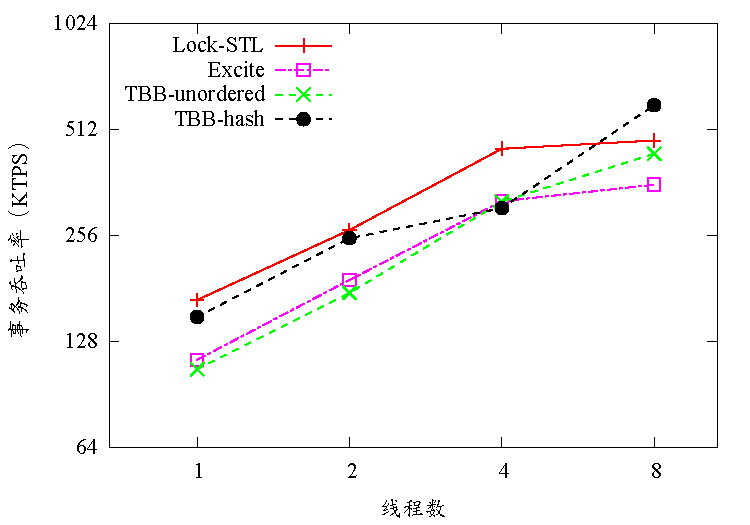
\includegraphics[width=0.8\linewidth]{workloada}
  \caption{YCSB中负载A测评结果。}
  \label{fig:workload-a}
\end{figure}

\begin{figure}[!ht]
  \centering
  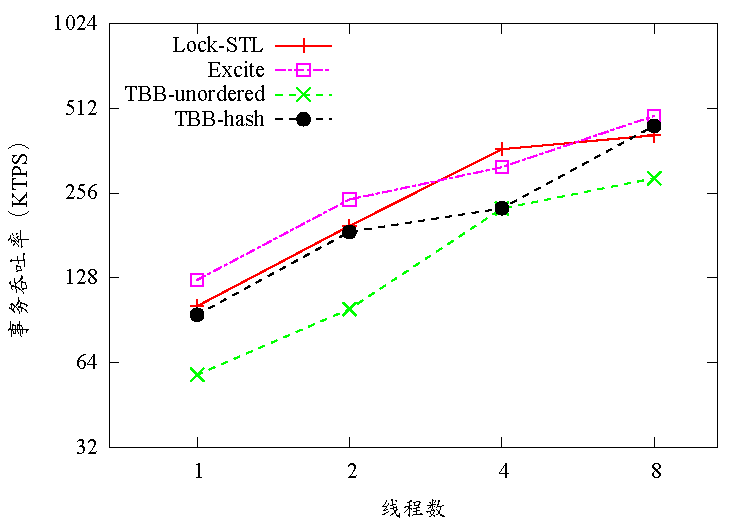
\includegraphics[width=0.8\linewidth]{workloadb}
  \caption{YCSB中负载B测评结果。}
  \label{fig:workload-b}
\end{figure}

\begin{figure}[!ht]
  \centering
  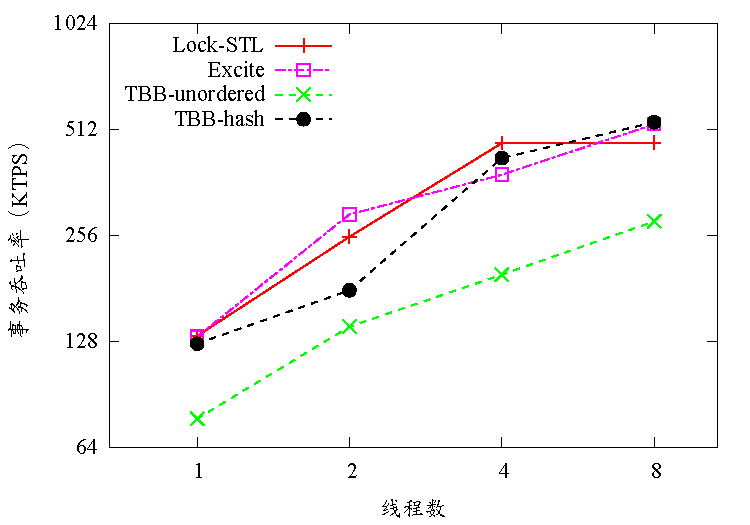
\includegraphics[width=0.8\linewidth]{workloadc}
  \caption{YCSB中负载C测评结果。}
  \label{fig:workload-c}
\end{figure}

\begin{figure}[!ht]
  \centering
  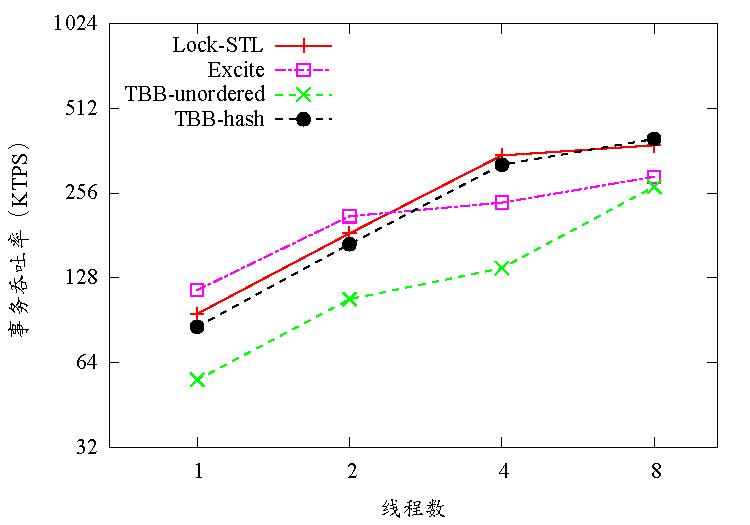
\includegraphics[width=0.8\linewidth]{workloadd}
  \caption{YCSB中负载D测评结果。}
  \label{fig:workload-d}
\end{figure}

\begin{figure}[!ht]
  \centering
  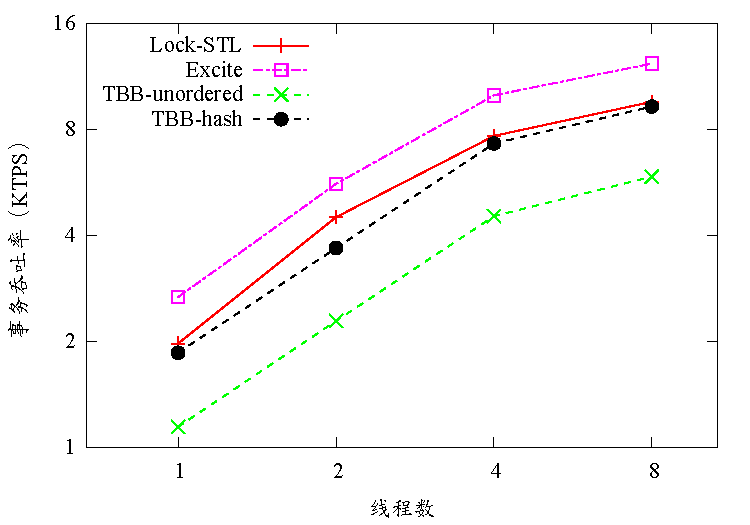
\includegraphics[width=0.8\linewidth]{workloade}
  \caption{YCSB中负载E测评结果。}
  \label{fig:workload-e}
\end{figure}

\begin{figure}[!ht]
  \centering
  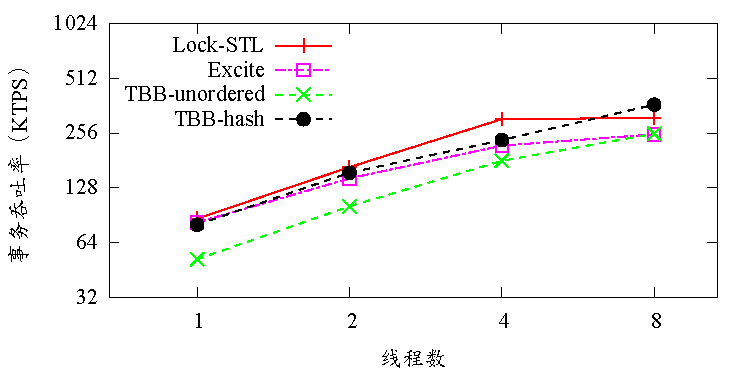
\includegraphics[width=0.8\linewidth]{workloadf}
  \caption{YCSB中负载F测评结果。}
  \label{fig:workload-f}
\end{figure}

通过这些数据,我们可以得出两点观察结论。第一,基于英特尔线程库TBB中concurrent\_unordered\_map实现的键值存储平均性能最优。我们的系统很难完全超越TBB,主要在于快照隔离在验证等方面的效率瓶颈。第二,当开启8个客户线程的时候,我们的系统比BTT最优实现的吞吐率低13.3\%,但是在读操作密集的负载下,我们的系统比BTT最优实现的吞吐率高32.5\%。这体现出快照隔离设计对日益重要的读写混合负载的高效支持。

更新的测评结果参见项目开源网站\url{http://persper.com/libptm}。

\section{本章小结}

总结起来,本章工作主要从三个方面推进了事务性内存接口下的持久性数据一致性机制。第一,我们提出了持久性事务性内存模型,为传统事务性内存增添了高效的持久性保证,将大容量的非易失性存储\emph{直接地}交由应用访问。第二,利用了我们事务性内存系统快照隔离的特性,将持久化的开销从只读负载的关键路径中移除。第三,考虑SSD和NVMe接口特性,设计了新的日志机制,小缓冲区组技术,同时达到高吞吐率和低延迟。


